


\graphicspath{{chapters/paper4/}}


\chapter{Paper 4}
{\Huge \textbf{Assessment of regional myocardial work from a patient-specific
  cardiac mechanics model}}

% \clearpage
\newpage
\section*{Assessment of regional myocardial work from a patient-specific
  cardiac mechanics model}

% \begin{center}
  Henrik Finsberg$^{1,2,3}$,
  John Aalen$^{2,5}$,
  Camilla K. Larsen$^{2,5}$,
  Espen Remme$^{2,5}$,
  Joakim Sundnes$^{1,2,3}$,
  Otto A. Smiseth$^{2,5}$, and
  Samuel Wall$^{1,2,4}$,
% \end{center}

% \onehalfspacing
\footnotesize
\begin{enumerate}[itemsep=-2mm]
\item{Simula Research Laboratory, Lysaker, Norway}
\item{Center for Cardiological Innovation, Oslo, Norway}
\item{Department of Informatics, University of Oslo, Oslo, Norway}
\item{Department of Mathematical Science and Technology, NMBU, \r{A}s,
    Norway}
\item{Institute for Surgical Research, Oslo University Hospital, Oslo,
    Norway} 
\end{enumerate}
\normalsize
 

\subsection*{Abstract}
  Subject-specific computational models of heart mechanics, calibrated
  to replicate clinically measured motion data, can be used to
  estimate regional myocardial work, and thereby provide a measure of
  regional function and dysfunction.

  Finite element models of human left ventricles (LV) of one healthy
  case and one patient diagnosed with left bundle branch block (LBBB)
  were fitted to clinical data consisting of LV volume, regional
  longitudinal strain, and non-invasive estimates of LV pressure. Excellent
  fit between measured and simulated observations was obtained by means
  of gradient-based minimization of model-data mismatch.
  
  Regional myocardial work was assessed using several approaches,
  including the area of pressure-strain loops and the area of fiber stress-strain
  loops. Qualitative indices of efficiency and quantitative measures of
  mechanical power density were compared using the different approaches,
  including the well established pressure-volume area.

  Results show that the different approaches for computing regional
  work are qualitatively similar, and are able to capture regional
  dysfunction. However, the different approaches are quantitatively
  very different, and total mechanical work computed using the finite
  element model are in close agreement with the actual stroke work.

  In conclusion, mechanical work computed using a personalized cardiac
  mechanics model is quantitatively similar to the actual mechanical
  work estimated by the area of the pressure-volume loop. This allows
  for potentially non-invasive quantitative assessment of regional
  myocardial work, and would greatly improve diagnostics of patients
  with regional dysfunction, such as dyssynchronous heart failure. 


\section{Introduction}



% Left ventricular (LV) systolic function is commonly quantified
% using global indices such as ejection fraction or QRS-width. However,
% these are global measures that does not take into account that regional
% dysfunction, such as dyssynchrony, might be present.

Patients suffering
from left ventricular dyssynchrony, such as in the 
case of left bundle branch block (LBBB), might experience an inefficient pumping
of blood due to uncoordinated contraction of different
segments in the heart. Cardiac Resynchronization Therapy (CRT) is
a well established treatment option for these patients \cite[Section
8.2]{ponikowski20162016}. However, 30-40 \% of patients selected for
this treatment do not respond positively, indicating that the current
selection criteria are sub-optimal, and that new biomarkers are needed
for improving the current clinical practice. 

Typically for LBBB is that septal segments are activated early,
causing a stretch of the opposing lateral wall. The 
contraction of the late-activated lateral wall then results in a 
lengthening of the septal segments during systole, which can be
identified as wasted work. Recent studies 
\cite{vecera2016wasted} have shown that wasted septal work due to the
uncoordinated contraction might be a better predictor for response to
CRT, and that the amount of wasted work reflects the potential for
recovery. In these calculations, regional work is computed as the area
of the pressure-strain loops, where regional longitudinal strain is
measured using speckle tracking echocardiography (SPE), and left
ventricular pressure (LVP) is estimated using a non-invasive method
\cite{russell2012novel}. The same approach, though with other ways of
assessing regional strain and LVP, has been used in earlier studies to
quantify regional myocardial work
\cite{tyberg1974analysis,theroux1974regional}. These calculations are
inspired by the well established correlation between pressure-volume
(PV) area and myocardial oxygen consumption \cite{suga1979total}.
%  the
% area bounded by the end-systolic PV line, the systolic limb of the PV
% loop trajectory and the volume-axis,

% Total mechanical energy computed using a time-varying elastance model
% show strong correlation with cardiac oxygen consumption
% \cite{suga1979total}. Moreover, in the same study it was shown that
% under the assumtions stated in the time-varying elstance model, the
% energy consumtion of a real left ventricle was about twice as much as
% the total mechanical energy, suggesting that about 50 $\%$ of the
% energy is used for contractile purposes while the rest dissipate as
% heat.


Although the pressure-strain loop area as an estimate of regional
myocardial work has shown to be a useful metric in e.g predicting the
response to CRT, it suffers from limitations when compared to computation of 
``real'' myocardial work. Intraventricular pressure is
used as a surrogate for stress, because stress is not possible to
directly measure in an intact heart
\cite{huisman1980measurement}. Consequently, in these calculations all
segments are assumed to be subjected to the same stress, regardless of
differences in overall size, curvature or wall thickness.  

% These limitations have been evaluated by Skulstad et al
% \cite{skulstad2002postsystolic}, who computed regional work
% based on longitudinal strain and estimated wall stress using the law of
% Laplace, which accounts for the wall thickness and radius of
% curvature. They found essentially the same results when compared to
% estimates using the cavity pressure as surrogate for stress.

These limitations have been evaluated by Delhaas et. al
\cite{delhaas1994regional} who showed that
the area of regional fiber stress-strain loops was correlated to
regional oxygen demand in six canine left ventricles. In this study,
regional fiber stress was estimated based on assumptions of rotational
symmetry \cite{arts1991relation}, with each segment scaled according to
measured fiber strain. Fiber strain was measured at the subepicardial
layers using a two-dimensional video technique.


However, several simplifications, in particular regarding symmetry, is
made in these simplified models \cite{zhang2011comparison}, and the
measurement has to be done {\it in situ}.

Finite element models offer a safe and accurate way assessing
regional myocardial work {\it in vivo}, through mechanics models
constrained with clinical data \cite{balaban2017high}. This approach
allows for formulation of proper constitutive relations
\cite{holzapfel2009constitutive}, and realistic ventricular geometries
and fiber architecture. Hence, more realistic estimates of fiber
stress can be computed and fiber strain can be estimated through the
wall and are therefore not limited only to the subepicardial layers. 

% Approaches involving simple approximations of ventricular fiber or
% wall stress assumes symmetric properties of the left ventricle, and
% homogeneous distribution of fiber stress. These assumptions are vital
% in terms of stress estimation, and are known to cause
% discrepancy between stresses computed using Laplace-type laws and
% stresses computed in a finite element model
% \cite{zhang2011comparison}.


Wang et al \cite{wang2011myocardial} used displacements from
tagged MRI to estimate a single set of material parameters and a
time-varying active tension in a finite element model of five
canine left ventricles. These parameterized models were used to assess
regional myocardial work using an approach outlined in
\cite{niederer2009role}, and they found large regional variations.


However, a framework for assessing regional estimates of myocardial
work, for which, when all regions are considered, sums up to the total
stroke work needed to eject blood to the body, is still
lacking. Furthermore, in order to be clinically useful, the framework
has to be accurate in terms of being able to replicate the mechanical
conditions observed clinically, and fast in terms of computing these
estimates within a reasonable time frame.

In this study we apply a recently developed framework
\cite{balaban2017high} for constraining a mechanical model to clinical
data. This framework employ gradient-based optimization to estimate high
dimensional parameters in order to minimize the model-data mismatch,
and therefore offers the needed accuracy. Moreover, the framework
utilizes state-of-the-art numerical methods which computes the
gradient efficiently by solving the corresponding adjoint equation,
and thereby provides these estimates within a reasonable time frame. 

The result is a personalized cardiac mechanics model, that can used to quantify
regional myocardial work. We perform both a qualitative and a
quantitative analysis of the different methodologies to asses regional
as well as global measures of work. In particular we compare work
computed using a finite element model, with work computed as the area
of the pressure strain-loops, and also compare these results
to the total stroke work estimated by the area of the
pressure-volume loop.



\section{Methods}


\subsection{Mechanical modeling}
\label{sec:mechanical_modeling}
We represent the heart as a continuum body with a reference configuration 
$\Omega \subset \mathbb{R}^3$, and let $\Xvec$ denote the
corresponding reference coordinate. Further let $ \Omega_t
\subset \mathbb{R}^3$ be the deformed domain after a given time $t >
0$ and let $\xvec$ be the corresponding physical coordinate.  The
motion of a point $\Xvec \in  \Omega$ to the  point $\xvec \in
\Omega_t$ may be described by a deformation map  $\varphi :
\Omega  \rightarrow \Omega_t$. 

The deformation gradient associated with the motion $\xvec =
\varphi(\Xvec)$ is a rank-2 tensor given by 
\begin{align}
\F(\Xvec) = \frac{\partial \varphi}{\partial \Xvec},
\end{align}
and the deformed and reference configuration are related via the
displacement field  $\uvec$ by 
\begin{align}  
\uvec = \xvec-\Xvec = \varphi( \Xvec) -\Xvec.
\end{align}
Further, we introduce the determinant of the deformation gradient, $J =
\det \F$, and the right Cauchy-Green deformation tensor $\C = \F^T \F$.

The myocardium is modeled as a hyperelastic material, and we adapt a
transversely isotropic law from \cite{holzapfel2009constitutive},
where the strain-energy function $\Psi$ is given by  
\begin{align}
  \label{eq:hoa}
  \Psi(\Cbar) = \frac{a}{2 b} \left( e^{ b (\bar{I}_1  - 3)}  -1 \right)
  + \frac{a_f}{2 b_f} \left( e^{ b_f (\bar{I}_{4\ef} - 1)_+^2} -1 \right). 
\end{align}
Here $\bar{I}_1 = \tr \Cbar$ and $\bar{I}_{4\ef}= \ef \cdot (\Cbar
\ef)$ with $\Cbar = J^{-2/3}\C$ being the isochoric part of the right
Cauchy-Green deformation tensor , $\ef$ is a
unit vector field in the direction of the myofibers, $(\cdotp)_{+} 
= \max\{\cdot, 0\}$, and $a, a_f, b, b_f$ are 
material stiffness parameters defining the elastic properties of the
myocardium.

Incompressibility is forced by using a two-field variational approach
where the term
\begin{align}
\Psi_{\text{vol}} = - p (J-1), 
\end{align}
is added to the total strain energy density, and the variable $p$ is
introduced as a Lagrange multiplier.

To model the active contraction of the ventricle we employ the active
strain formulation. In this formulation one assumes a multiplicative 
decomposition of the deformation gradient into an elastic
and an active component \cite{ambrosi2011electromechanical}:
\begin{equation}
 \F = \F_e \F_a.
\label{eq:active_strain}
\end{equation}
The active part, $\F_a$ represents the active shortening of the cells,
while the elastic part $\F_e$ ensures compatibility of the tissue.
Similar to \cite{balaban2017high} we choose the following form of the active
deformation gradient,
\begin{equation}
  \F_a = (1 - \gamma) \ef \otimes \ef  + \frac{1}{\sqrt{1 - \gamma}} (\I - \ef \otimes \ef).
 \label{eq:active_strain_Fa_gjerald}
\end{equation}
The active deformation gradient $\F_a$ does not contribute to any
stored energy within the material, so that the modified
strain-energy function $\tilde{\Psi}(\C_e) = \Psi(\F_a^{-T} \Cbar
\F_a^{-1})$, which is a pure function of the elastic deformations is used.

The force balance equation can be derived from the classical Cauchy
momentum equation, and with the assumption that the inertial term and
external body forces are negligible, the strong formulation yields
\begin{align}
  \nabla \cdot \FPiola &= 0, \\
  J &= 1, 
\end{align}
with $\FPiola = \frac{\partial \Psi}{\partial \F}$ being the first
Piola-Kirchhoff stress tenors. 

To solve the problem we employ the Galerkin finite element method, which is based
on choosing proper finite dimensional subspaces $V_h \subset [H_0^1(\Omega)]^3$ and
$Q_h \subset L^2(\Omega)$ and solve the weak formulation of the problem. In
the Lagrangian form, the weak form reads: {\it find $(\uvec,p)
\in V_h\times Q_h$ such that for all variations $(\delta
\uvec, \delta p) \in V_h \times Q_h $ and $\left. \left( \uvec \cdot \N \right)
\right|_{\partial \Omega_{\mathrm{base}}} = 0$ }:
\begin{align}
\begin{split}
  F(\uvec, p;\delta \uvec, \delta p) =
  &\int_{\Omega} \FPiola :  \Grad \delta \uvec  \mathrm{d} V  \\
  &+\int_{\Omega} p J \F^{-T} : \Grad \ \delta \uvec   \mathrm{d} V  
  +\int_{\Omega} (J - 1) \delta p \mathrm{d} V \\
  &+\int_{\partial \Omega_{\text{base}}} k \uvec \cdot \N \mathrm{d}S
  - \int_{\partial \Omega_{\text{endo}}} \plv J \F^{-T} \N \cdot \delta \uvec \mathrm{d}S= 0.
  \label{eq:force_balance}
\end{split}
\end{align}
Here, the ventricular domain is anchored by constrained the basal
motion by a linear spring-term with stiffness $k$, and the
endocardial cavity pressure $\plv$ is enforced as a Neumann boundary
condition on the endocardium.  

For discretization we use the so called Taylor-Hood finite elements,
which is known to yield a stable discretization for this problem
\cite{arnold1984stable}. These elements consist of quadratic finite
elements for the displacement, and linear finite elements for
the hydrostatic pressure. 



\subsection{Calculation of work}
\label{sec:regional_work}

Work can be computed by considering any of the
work conjugate stress-strain pairs \cite{holzapfel2000nonlinear}. In
the current configuration it is common to use the Cauchy stress tensor
$\Cauchy = \FPiola \F^T$ and the Almansi strain tensor $\mathbf{b} =
\frac{1}{2} \left(\I -  \F^{-T} \F^{-1} \right)$, while in
the reference configuration we use the second Piola-Kirchhoff stress
tensor $\SPiola = \F^{-1} \FPiola$, and the Green-Lagrange strain
tensor $\E = \frac{1}{2}\left(\C - \I \right)$. Thus, in the Lagrangian
description, the total mechanical work from time $t_1$ to $t_2$ in a
region $\Omega_j$ is given by
\begin{align}
   \mathcal{W}(t_1, t_2)[\Omega_j] = 
  -\int_{t_1}^{t_2} \int_{\Omega_j}\SPiola(t, \Xvec)
  : \dot{\E}(t, \Xvec) \mathrm{d}\Xvec \mathrm{d}t, 
\end{align}
where $ \dot{\E} $ is the rate of the Green-Lagrange strain tensor.
By dividing by the volume of the region of interest $| \Omega_j |$,
we obtain the average work density in that region. Note the sign
convention used here illustrates that a negative strain-rate
represents positive work. To only compute the
work along a specific direction, e.g along the fibers, the full stress
and strain tensors are simply interchanged with their respective
components in that direction, and the double contraction of the tenors
is changed to a scalar multiplication.

The mechanical work needed to eject blood from time $t_1$ to
$t_2$ is given by
\begin{align}
   \mathcal{W}(t_1, t_2)[\Omega] = 
  -\int_{t_1}^{t_2} \frac{\mathrm{d}V}{\mathrm{d}t} P(t) \mathrm{d}t,
\end{align}
where $V(t)$ and $P(t)$ refers respectively to the cavity volume and pressure in
the left ventricle $\Omega$ at time $t$. If the $t_1$ and $t_2$
represents respectively the start and end of the cycle, then normalizing with respect to the
total ventricular wall volume  $| \Omega |$, would yield a measure of
total mechanical work density (TMWD). Diving the TMWD by the total
cycle time, would yield a measure of total mechanical power
density (TMPD). We note that for analysis of performance, TMPD is
a better measure than total work because it is independent of
morphology and heart rate.  

\subsubsection{Quasi-static approximation}
The mechanical model described in Section
\ref{sec:mechanical_modeling} is quasi-static, meaning that the
inertial forces are assumed to be so small that the
equilibrium equation \eqref{eq:force_balance} holds at any discrete
time point. Therefore, strain rate is estimated using a
backward difference approximation \cite{wang2011myocardial}.
Suppose we have $N$ discrete time points $t = 0,1, \cdots N$, where $ t = 0$
refers to the the reference configuration, and let $\SPiola(t, \Xvec)$
and $\E(t, \Xvec)$ be respectively the stress and strain tensors at
time $t$ and position $\Xvec$ in the reference configuration. In the
following, the full stress and strain tensors are used, but the methodology
also applies to any component of the stress and strain tensor. We define
\begin{align}
  \overline{\SPiola}(t,\Xvec) &= \frac{1}{2}\left( \mathbf{S}(t,\Xvec) + \mathbf{S}(t-1,\Xvec) \right),\\
  d\E(t,\Xvec) &= \E(t,\Xvec) - \E(t-1,\Xvec),
\end{align}
for $t = 1,\cdots, N$, and note that $ \mathbf{S}(0) = \mathbf{E}(0) = \mathbf{0}$.
The mechanical work in a region $\Omega_j$ from time $t=m$ to time $t=n$ can now be approximated
as 
\begin{align}
  \begin{split}
   \mathcal{W}(m, n)[\Omega_j]
  &= -\int_{t=m}^{t=n} \int_{\Omega_j}\SPiola(t, \Xvec) : \dot{\E}(t, \Xvec) \mathrm{d}\Xvec \mathrm{d}t \\
  &\approx - \sum_{t = m}^{n}\int_{\Omega_j}\overline{\SPiola}(t, \Xvec) : d\E(t, \Xvec) \mathrm{d}\Xvec
  \end{split}
\label{eq:total_work}
\end{align}
Similarly, the mechanical work computed from the pressure-volume loop area can be estimated as  
\begin{align}
  \begin{split}
  \mathcal{W}(m,n)[\Omega]
  &= - \int_{t=m}^{t=n} \frac{\mathrm{d}V}{\mathrm{d}t} P(t) \mathrm{d}t \\
  &\approx -\sum_{t = m}^{n}  (V(t) - V(t-1)) \cdot \frac{P(t) + P(t-1)}{2}.
  \end{split}
\end{align}

% Note that calculation of segmental work in Reference
% \cite{russell2013assessment} is exactly the same but with pressure
% used as a surrogate for stress and longitudinal strain used in stead of
% fiber strain. 

\subsubsection{Efficiency and wasted work ratio (WWR)}
\label{sec:efficiency_wwr}

During systole, most segments shorten and performs positive work
($\mathcal{W}_{\mathrm{pos}}$). However some segments might elongate,
resulting in energy loss, and we say that these segments do negative work
($\mathcal{W}_{\mathrm{neg}}$). Positive work is identified as the points with
$d\E_{\ef}(t) < 0$ (shortening), while negative work is identified as points with
$d\E_{\ef}(t) > 0$ (lengthening).
A local measure of the energetic efficacy of each segment is the ratio between the
negative and positive work, an index known as the segmental wasted
work ratio (WWR) \cite{russell2013assessment},
\begin{align}
  \mathrm{WWR} = \frac{|\mathcal{W}_{\mathrm{neg}}|}{\mathcal{W}_{\mathrm{pos}}}
\end{align}
Another measure of efficiency, formulated by Niederer et al
\cite{niederer2009role} is the ratio of positive work and the total
work
\begin{align}
  \eta = \frac{\mathcal{W}_{\mathrm{pos}}}{\mathcal{W}_{\mathrm{pos}} + |\mathcal{W}_{\mathrm{neg}}|}.
  \label{eq:efficiency}
\end{align}

The two indices are related as follows: $\eta = \left( 1 +
  \mathrm{WWR} \right)^{-1}$, and we will therefore only report values
of the efficiency \eqref{eq:efficiency}, for which a value close to 1.0 indicate that most
of the performed work is positive. Since we expect work during systole
to be the main contribution to the overall ejection of blood, this
index is computed by only including work done from mitral valve closing to
mitral valve opening \cite{russell2013assessment}. 

Note that with the current sign-convention, negative work is by
definition negative, which is why we take the absolute value of the
negative work. 

\subsection{Pre-processing of in vivo data sets}

In this study 4D echocardiographic images of one patient diagnosed
with left bundle branch block (LBBB) and one healthy volunteer was
acquired using a GE Vingmed E9 machine (GE Healthcare Vingmed, Horten,
Norway). 
The analysis of the echocardiographic images was conducted with the
GE software package EchoPac version 202. Longitudinal strain was
measured via speckle tracking echocardiography (SPE) in the 17 AHA segments
\cite{cerqueira2002standardized}. However, the apical segments for both
subjects as well as the inferior and posterior basal segment for the
normal case were excluded due to poor quality.

Using a semi-automatic image segmentation tool, the LV cavity volumes for
each frame was measured, and the LV endocardial and epicardial
surfaces were extracted from the image frame corresponding to
beginning of atrial systole \cite{hansegaard2009semi}. A cut was made
at the base of these surfaces so that the measured and computed cavity
volumes agreed within a tolerance of 1 ml. Thereafter, a left
ventricular tetrahedral mesh was created using Gmsh
\cite{geuzaine2009gmsh}. Myocardial fiber orientations were assigned
using the Laplace-Dirichlet Rule Based  (LDRB) algorithm
\cite{bayer2012novel} with an angle of $60^{\circ}$ on the endocardial
and $-60^{\circ}$ on the epicardial surface
\cite{streeter1969fiber}. A non-invasive method
\cite{russell2012novel} was used to estimate an LV pressure curve for
both subjects, so that all clinical data used in this study were
acquired using non-invasive methods. 


\subsection{Data assimilation and parameter estimation}

In order to constrain the mechanical model to clinical data, we
applied a variational data assimilation technique. Let $\mathbf{w} =
(\uvec,p)$ denote a joint state variable consisting of the
displacement field $\uvec$ and the hydrostatic pressure $p$. The LV
cavity volume can be approximated as  
\begin{align}
  \mathcal{H}_{\mathrm{volume}}(\mathbf{w})= -\frac{1}{3}\int_{\lvendo}
  \left( \Xvec + \uvec \right) J \F^{-T} \Nvec \mathrm{d}S, 
  \label{eq:volume_operator}
\end{align}
where $\N$ denotes the unit facet normal. Furthermore, the average regional
longitudinal strain can be approximated in region number $j$ as
\begin{align}
  \mathcal{H}_{\mathrm{strain}, j}(\mathbf{w}) = \frac{1}{|\Omega_j|}\int_{\Omega_j}
  \mathbf{e}_l^T \left( \mathbf{\tilde{\F} - \I} \right)\mathbf{e}_l  \mathrm{d}V.
\end{align}
Here $\mathbf{e}_l$ denotes a unit vector field in
the longitudinal direction, and $\tilde{\F}$ refers to the modified deformation
gradient relative to the reference geometry in the measurements. 

For a given measurement $y_k$, we want to find a state variable
$\mathbf{w}$ that minimizes the mismatch between $y_k$ and
$\mathcal{H}_k(\mathbf{w})$. The state variable is determined by
tuning model-based parameters, also
referred to as control parameters, which we generically denote
by $\mu$. This can be formulated as a PDE-constrained optimization
problem of the form
\begin{equation}
  \begin{aligned}
    \label{eq:pde_opt}
    & \underset{\mu}{\text{minimize}}
    & &  \mathcal{J}(\mathbf{w}(\mu), \mu) \\
    & \text{subject to}
    & & F(\mathbf{w}, \mu)  = 0,
  \end{aligned}
\end{equation}
where $F=0$ represents the PDE-constraint given by
\eqref{eq:force_balance}, and $\mathcal{J}$ is a possibly
multiobjective function  
\begin{align}
  \mathcal{J}(\mathbf{w}(\mu), \mu) = \sum_{k = 1}^{N} w_k j_k (\mathbf{w}(\mu), \mu),
  \label{eq:cost_functional}
\end{align}
with $w_k$ being scalar weights, and $j_k = d( y_k,
  \mathcal{H}_k(\mathbf{w}) ) $ for some suitable metric $d$.



\subsubsection{Joint estimation of unloaded configuration and passive
  material parameters}
\label{sec:passive_param_estim}

One challenge when using image-based geometries is that the geometry
observed in a medical image is subjected to loads, e.g blood
pressure, while our finite element formulation assumes a stress-free
reference configuration. Therefore we need to find a geometry, so
that when the measured pressure in the image is applied, we recover
the image-based geometry. Several methods for estimating the unloaded,
zero-pressure geometry exist, including the inverse design analysis
(ID) \cite{govindjee1996computational}, the modified updated
Lagrangian formulation (MULF) \cite{gee2010computational} and
iterative methods \cite{bols2013computational,Rausch2017JB}.
Here we apply a simple fixed-point iteration scheme known as the backward
displacement method \cite{bols2013computational}.
The estimated unloaded configuration will depend upon the choice of material
parameters, which is not know  \emph{a priori}. In Appendix
\ref{sec:unloading} we explain the main steps in the backward
displacement method and a proposed method for joint estimation of material
parameters unloaded configuration. Additionally, an analysis of
the convergence properties of this method is also provided.


\subsubsection{Active parameter estimation}
\label{sec:active_param_estim}
From the first measurement point after end-diastole and throughout the
remaining cardiac cycle, that parameter $\gamma$ in
\eqref{eq:active_strain_Fa_gjerald} is used as control in
\eqref{eq:pde_opt}, and the cost functional \eqref{eq:cost_functional}
at time point $i$ is given by 
\begin{align}
  \mathcal{J} =
   \left(\frac{\mathcal{H}_{\mathrm{volume}}(\uvec^i)
  - V^i}{V^i} \right)^2 +
  \sum_{j=1}^{12} \delta_j \left( \mathcal{H}_{\mathrm{strain}, j}(\uvec^i)
  - \varepsilon_{j}^i \right)^2  + \lambda \| \nabla \gamma \|^2.
\end{align}
Here $V^i$ is the measured cavity volume at time point $i$, 
$\varepsilon_{j}^i$ is the measured longitudinal strain in segment $j$
at time point $i$, and $\delta_j$ is 0 if the measurement in segment
$j$ is missing and 1 otherwise. Note that even though the  
AHA-representation \cite{cerqueira2002standardized} contains 17
segments, we only include the mid and basal segments in the
optimization because of the relatively poor quality of the apical
segments, leaving us with a total of 12 segments.

The parameter $\gamma$ is represented as a piecewise linear function
with one parameter per vertex as suggested in \cite{balaban2017high}.
This problem is therefore highly under-constrained, meaning that there
are potentially many solutions to problem. To remedy this we apply a
Tikhonov regularization, where we penalize non-smooth values of the
control by adding the term $\lambda \| \nabla \gamma \|^2$ to the
objective functional. The regularization parameter $\lambda$
was chosen based on a previous study to be $\lambda=0.01$ \cite{balaban2017high}.

At each point the optimal value of the previous point is used as
initial guess, and zero for the first point of active contraction.


\section{Results}
For the normal and LBBB case defined above, we ran the
full pipeline on two meshes, where one was a refined version of the
other. For the normal case, the original and refined mesh had
respectively 2569 and 5258 elements, while the LBBB case
had 2572 elements in the original mesh and 5114 elements in the
refined mesh. Results on the original and refined geometries gave
close to identical results, and we will therefore only present the
results using the coarsest geometry. 

All simulations were carried out using an in-house software
package\footnote{Source code is publicly available at
  \url{https://bitbucket.org/finsberg/pulse_adjoint}} 
based on FEniCS \cite{logg2012automated} and Dolfin-Adjoint \cite{farrell2013automated}.
In these simulations the value of the linear spring $k$ in
\eqref{eq:force_balance} was determined by testing a range of values,
and choosing the softest spring that allowed for a convergent
estimation of the unloaded configuration. Based on this experiment we
choose $k=0.01$ kPa/cm$^2$.

During the estimation of the active and passive parameters outlined in Section
\ref{sec:active_param_estim} and \ref{sec:passive_param_estim}
respectively, the optimization was terminated if the value between two
successive iterations was less then $10^{-6}$ or the number of
iterations exceeded 100. For the material parameter, an upper and lower
bound was set to $50$ and $0.05$ kPa respectively, while for the active
parameter these bounds were set to $0.4$ and $0.0$, allowing for up to
40 $\%$ active shortening of the myofibers. 



% \subsection{Estimation of unloaded configuration and passive material
%   parameters}

% The linear isotropic material parameter $a$ in \eqref{eq:hoa}, along
% with an unloaded configuration was estimated by means of Algorithm
% \ref{alg:unload_mat_bdm} for both the normal and the LBBB case.
% Figure \ref{fig:unloaded_simulation} shows the value of the material
% parameters, and the residual representing the relative difference
% between the unloaded cavity volumes of two successive iterations.
% The LBBB and normal case used respectively
% $7$ and $17$ iterations to get the residual below 0.01, resulting in a
% material parameters of $a= 32.1$ kPa for the LBBB case and $a= 11.96$ kPa for the
% normal case.
% \begin{figure}[htbp]
%   \centering
%   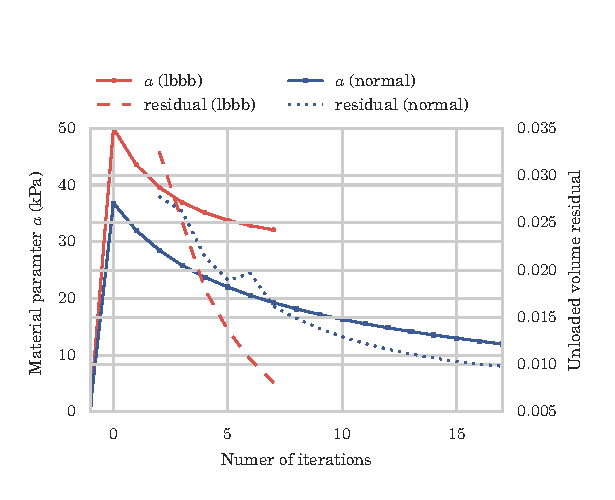
\includegraphics{figures/unloaded_simulation}
%   \caption{\label{fig:unloaded_simulation}Estimation of material
%     parameters for normal (blue) and LBBB (red) case. Solid lines
%     show the value of the material parameter at each iteration with
%   initial guess in both cases being $a=1.291$ kPa (iteration -1). Then
% the offset of the pressure in the image-based geometry was subtracted
% and new material parameters was estimated (iteration 0), and Algorithm
% \ref{alg:unload_mat_bdm} was applied using this estimate as initial
% guess. Dashed lines are the residuals, representing the relative
% difference in unloaded cavity volume. The algorithm terminated when
% the residual was below 1 \%. }
% \end{figure}
% Figure \ref{fig:unloaded_geo} shows the resulting
% unloaded configurations on top of the original geometries. 
% \begin{figure}[htbp]
%   \centering
%   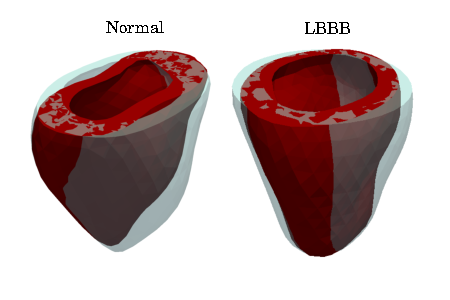
\includegraphics{figures/unloading}
%   \caption{\label{fig:unloaded_geo}Estimated unloaded
%     configuration for normal (right) and LBBB (left) case in red, and
%     the original image-based geometry in transparent. }
% \end{figure}


\subsection{Data assimilation}

The simulated and measured PV loops and the regional
pressure-strain loops are shown in Figure \ref{fig:pv_loops} and
\ref{fig:regional_strain_pressure_loops} respectively. 
For the normal case, the longitudinal strain curves in the basal
inferior and posterior segments were missing, and so only the
simulated results are shown in these segments.

\begin{figure}[htbp]
  \centering
  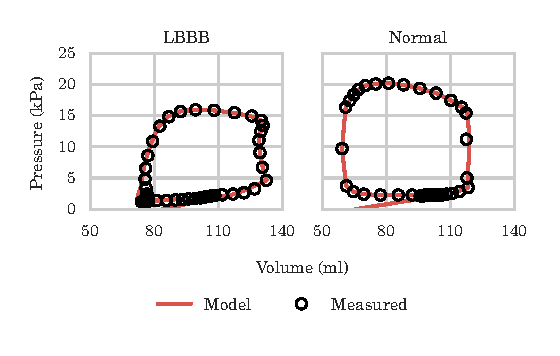
\includegraphics{figures/pv_loop}
  \caption{\label{fig:pv_loops}Simulated and measured PV loops
    for the LBBB (left) and normal (right) case. }
\end{figure}

In both the normal and the LBBB case, the
largest deviation between the measured and simulated volumes were found
during the end of isovolumic relaxation, where simulated volumes were
respectively at most 1.0 and 6.0 ml lower than the measured volumes.


\begin{figure}[htbp]
  \centering
  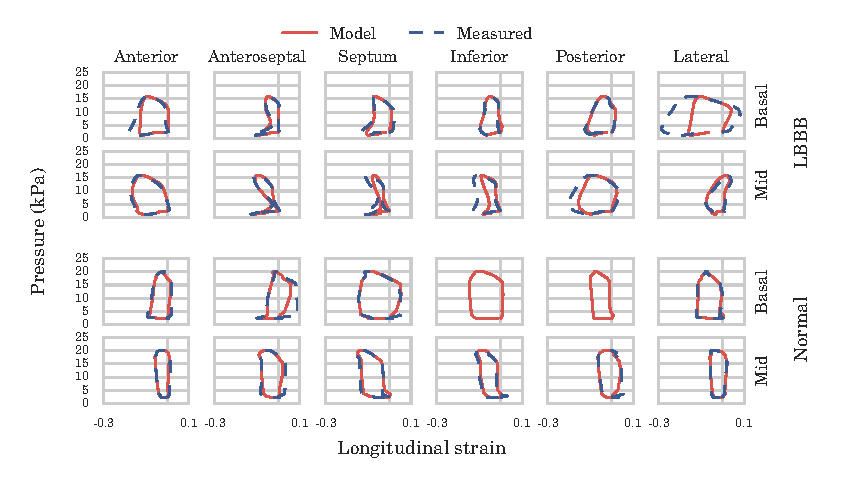
\includegraphics{figures/pressure_strain_loop}
\caption{\label{fig:regional_strain_pressure_loops}Measured and
simulated pressure-strain loops for LBBB (top) and normal (bottom)
case. Strain measurement in basal inferior and posterior segments for
the normal subject were discarded in the optimization due to poor
quality, and therefore only simulated results are shown in these
segments.} 
\end{figure}



\subsection{Estimation of regional myocardial work}

Analogous to the regional pressure-strain loops in Figure
\ref{fig:regional_strain_pressure_loops}, the resulting regional fiber
stress-strain loops are depicted in Figure
\ref{fig:regional_fiber_stress_strain_loops}. Here we show Cauchy
fiber stress on the $y-$axis and for the sake of correct illustration
of regional work in terms of loop area, we show the Almansi fiber
strain on the $x-$axis. 

\begin{figure}[htbp]
  \centering
  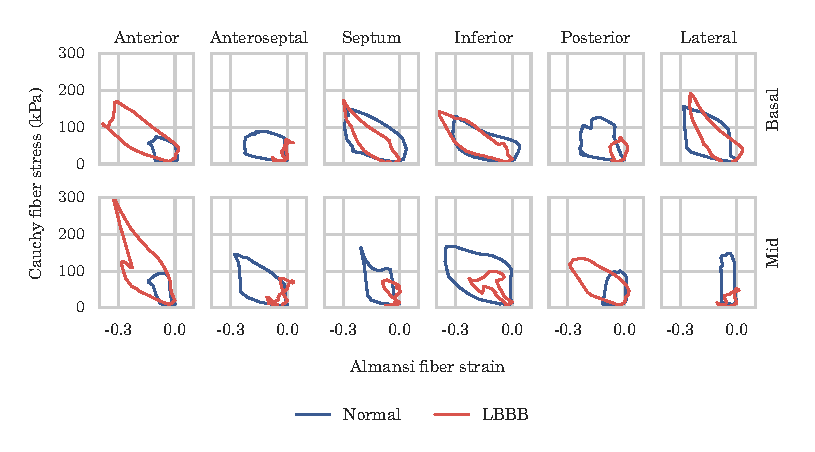
\includegraphics{figures/fiber_stress_strain_loop}
  \caption{\label{fig:regional_fiber_stress_strain_loops}Simulated
    regional fiber stress-strain loops in the mid and basal segments
    for normal (blue) and LBBB (red). } 
\end{figure}

The Cauchy fiber stress visualized at the deformed configurations at
the different valvular events for the normal and LBBB case are shown
in Figure \ref{fig:snap_shots}. The LBBB case shows clear signs of
dyssynchrony and more uneven distribution of stress compared to the
normal case. 

\begin{figure}[htbp]
  \centering
  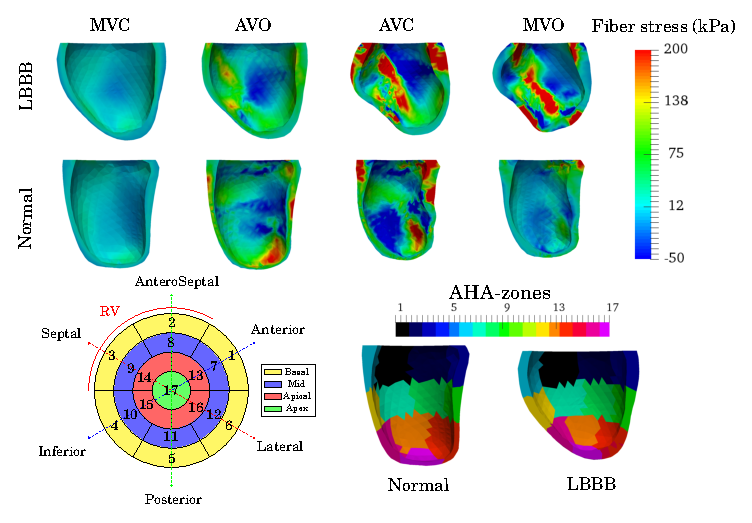
\includegraphics{figures/snap_shots}
  \caption{\label{fig:snap_shots}Cauchy fiber stress for the normal and LBBB case at
    different valvular events (MVC: mitral valve closing, AVO: aortic
    valve opening, AVC: aortic valve closing, MVO: mitral valve
    opening), visualized on the deformed configurations. For reference
    we show the 17 AHA-zone delineation of the left ventricle in the
    two cases in the bottom panel. From left to right we have the
    lateral, anterior, anteroseptal and septal segments. }
\end{figure}




The total mechanical power density (TMPD) is also computed using four
different approaches: 1) area of the pressure-volume loop normalized
to ventricular wall volume, 2) using the full stress and strain tensors,
3) using the fiber component of the stress and strain tensors, and 4)
using global longitudinal strain and estimated pressure. Table
\ref{tab:total_mechanical_power} show these values for the two
patients, in units kW m$^{-3}$. In the calculations of pressure volume
area, the simulated volume is used, with the unloaded volume and zero
pressure included as reference point.

\begin{table}
\caption{Total mechanical power density (TMPD) computed using the area
  of the pressure-volume loop normalized to ventricular wall volume
  (PV area), the full stress and strain tensors (Full), the fiber
  component of the stress and strain tensors (Fiber) and using global
  longitudinal strain and estimated pressure (Pressure-GLS)} 
\begin{tabular}{lrrrr}
\hline
 Case   &   PV area (kW m$^{-3}$) &   Full (kW m$^{-3}$) &   Fiber (kW m$^{-3}$) &   Pressure-GLS (kW m$^{-3}$) \\
\hline
 LBBB   &                    8.41 &                10.60 &                  6.42 &                         1.02 \\
 Normal &                   15.79 &                16.35 &                  9.59 &                         1.59 \\
\hline
\end{tabular}
\label{tab:total_mechanical_power}
\end{table}

The regional TMPD, computed using the fiber
component of the stress and strain tensor, is illustrated for the mid
segments for the two subjects in Figure
\ref{fig:regional_power_density}. These regional values are
effectively the area of the fiber stress-strain loops in Figure
\ref{fig:regional_fiber_stress_strain_loops} normalized to cycle
time, in which the area is positive when the loop follows an
anti-clockwise orientation and negative if the loop has a clockwise
orientation. Regional TMPD using the full stress and strain tensor are
not shown, but were qualitatively similar to the regional TMPD using
only the fiber component.


\begin{figure}[htbp]
  \centering
  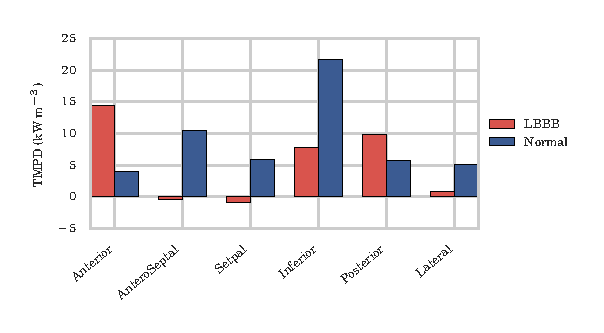
\includegraphics{figures/regional_power_density}
  \caption{\label{fig:regional_power_density} Regional TMPD in the mid
    segments for LBBB (left) and normal (right), computed using the
    fiber component of stress and strain tensors. Height of each bar
    indicate the area of the respective fiber stress-strain loop
    traversed in an anti-clockwise orientation, and normalized to
    cycle time.}  
\end{figure}

A qualitative comparison of the pressure-strain loops and fiber
stress-strain loops are illustrated in Figure
\ref{fig:regional_work_indices}, where we plot the regional efficiency
\eqref{eq:efficiency} using the two measures of work. We note that the
efficiency computed using the fiber stress-strain loops are
lower than for the pressure-strain loops but show the same trend, i.e
that regions with reduced efficiency coincide.  

\begin{figure}[htbp]
  \centering
  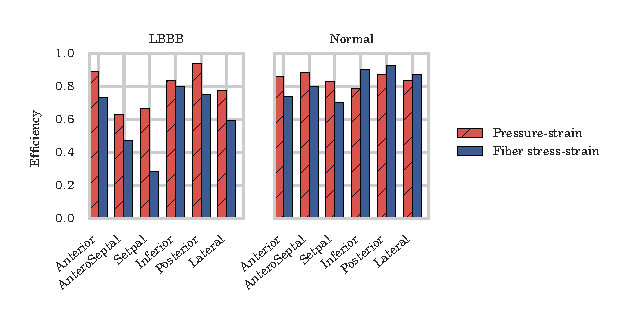
\includegraphics{figures/regional_work_indices}
  \caption{\label{fig:regional_work_indices} Regional efficiency in
    the mid segments computed according to \eqref{eq:efficiency} for LBBB (left) and normal (right)
    case. Red bars show efficiency based on areas of the pressure
    strain loops while blue bars show efficiency based on areas of the
    fiber stress-strain loops.}
\end{figure}


% \input{result_figures}
\section{Discussion}
In the present study, we have demonstrated how computational cardiac
modeling and data assimilation can be used to asses regional
myocardial work. The in vivo data sets making up these results are
based on echocardiographic images and non-invasive estimates of LV
pressure in one patient diagnosed with LBBB and one healthy volunteer. 
A gradient-based optimization method was used to minimize the mismatch
between the simulated and observed clinical data, so that the simulated
longitudinal strain and volume were quantitatively similar to the
measured values.

% In both cases an excellent fit of the PV loops was
% obtained, as can be seen in Figure \ref{fig:pv_loops}. The deviation
% between simulated and measured volume during late isovolumic
% relaxation shows that there is a trade-off between fitting both the
% strain and volume data. This can also be seen from the matching of the
% pressure-strain loops in Figure
% \ref{fig:regional_strain_pressure_loops}, where it is clear the some
% segments (e.g mid posterior and basal lateral) for the LBBB patient
% does not match exactly during the isovolumic relaxation phase. Whether
% this is a result of lack of mode fidelity, poor data compatibility, or
% just noise in the measurements is difficult to say.



\subsection{Pressure-strain versus fiber stress-strain}

The total mechanical work can be computed by considering the work done
by all segments during one full cardiac cycle. Ideally, we would have
a regional measure so that adding together all regional contributions
would sum up to the actual stroke work needed to eject blood to the
body. Since the stroke work is strongly correlated with the myocardial
oxygen consumption \cite{suga1979total}, a regional meausure of work
that summed up to the total stroke work would be a good measure of
regional performance. 
% Total mechanical power density (TMPD),
% which is a measure of average total mechanical work normalized to
% cycle time, is presented in Table
% \ref{tab:total_mechanical_power} using four different approaches,
% namely, the PV area, the full stress and strain tensor, the fiber
% stress-strain loops and the pressure-strain loops.

The TMPD computed using the PV area, which is a true measure of stroke
work, falls between the values of TMPD computed using the full stress
and strain tensor and the TMPD computed using the fiber stress and
fiber strain. In other words, the amount of work needed to eject blood
to complete a cycle is greater that the amount of work done by the
myofibers, but bounded above by the total mechanical work. Since there
are no viscous terms in the model, the energy should be
conserved. However, energy loss due work against the basal boundary
constraint could explain the difference between stroke work and the
total mechanical work. Furthermore, the TMPD computed from fiber
stress-strain area here, are comparable with values in other studies
using canine left ventricles \cite{delhaas1994regional}, which reports
values of TMPD in the range from 0.5 to 12.5 kW m$^{-3}$. Note that
TMPD is a measure that is independent of morphology, i.e size of the
ventricle and heart rate, and therefore reflect the actual performance.

The values in Table \ref{tab:total_mechanical_power} indicate that the
total mechanical work performed in the direction of the fibers is
approximately 60 $\%$ of the 
total mechanical work computed by taking into account the full stress
and strain tensor (LBBB: 60.5 $\%$, normal:58.7 $\%$). Of course, the
amount of work performed in transverse direction of the fibers will depend upon the
particular form of the active deformation gradient in
\eqref{eq:active_strain_Fa_gjerald}. In the active stress approach on 
the other hand, where the total Cauchy stress tensor is additively decomposed into
active and passive contributions, it is common to add an active stress
in the transverse direction, which is also reported
experimentally \cite{lin1998multiaxial}. By assuming
a volume preserving active deformation gradient, the amount of
work in the cross fiber direction as computed here is about $40 \%$, a
value that has been used in other modeling studies using the active
stress approach \cite{sun2009computationally}.

The values of regional TMPD in the mid segments presented
in Figure \ref{fig:regional_power_density} show that the septal
segments for the LBBB patient actually consumes energy and yield a
negative TMPD. On the other hand, the healthy heart shows positive TMPD
in all segments and generally higher values than the LBBB heart.
Since the TMPD computed using stress and strain derived from the
underlying constitutive equation agrees very well with the TMPD
computed from the PV area there is reason to believe that the regional
TMPD reflects the actual regional performance, and future studies should
investigate how well these values correlate with regional myocardial
oxygen consumption. 

The TMPD computed using the pressure and global longitudinal strain loop
only accounts for a small fraction of the total mechanical power.
This indicates that quantitatively this is not a good measure of
myocardial work. However, the area of the pressure-strain loops have shown to be a good metric
of regional efficiency and a promising index for predicting response
to CRT \cite{vecera2016wasted}. From Figure
\ref{fig:regional_work_indices} we see the same trends in terms of efficiency and wasted
work can be seen regardless of how work is computed, namely that early
activated segments are less efficient and have a higher wasted work
ratio than the other segments for the LBBB case. Therefore, relative
comparison of segments using pressure-strain loops seems to give the
same picture as when using the fiber stress-strain loops. 
The pressure strain loops for the LBBB case all have an
anti-clockwise orientation, indicating generation of work in all
segments. On the other hand, the fiber stress-strain loops in the
septal segments show a clockwise orientation which is evidence of
work usage. In other words, the two approaches show the same
trend, but the effect of the wasted work is magnified in the fiber
stress-strain loops.  

% The presence of clockwise oriented loops is primarily due to the change
% from longitudinal strain to fiber strain, and not the change from
% pressure to fiber stress. Therefore the re

% Myocardial fiber architecture is more or less longitudinally oriented
% near the subepicardial and subendocardial layers
% \cite{streeter1969fiber}, and therefore longitudinal strain is a
% good approximation of fiber strain when considering the subepicardial
% and subendocardial layers. However near the midwall, myofibers are
% close to circumferential \cite{streeter1969fiber} and therefore this
% assumption is no longer valid. The complex fiber architecture makes it
% almost impossible to make good estimate of fiber strain through the
% wall, and finite element models are probably the only way to properly
% assess fiber strain trough the wall. 

Because of the basal boundary condition, stress estimates near the
base in the finite element model might not be reliable. Therefore we
will pay most attention to the stress 
estimates in the mid segments as these are not greatly influenced by
the boundary condition at the base. For the normal patient we see in
Figure \ref{fig:regional_fiber_stress_strain_loops} a
more or less uniform distribution of fiber stress with peak regional
averaged fiber
stress ranging from approximately 100 to 160 kPa. For the LBBB
patients we see a much larger spread in peak fiber stress. In
particular, we see lower stress in most segments, and high stress
in e.g the mid anterior segment which is adjacent to a segment with
low efficiency. In other words, an inefficient segment seems to
redistribute its load to neighboring segments in order to compensate
for the diminished efficiency. This leads to high concentration of
localized stresses which eventually could be responsible for pathological remodeling
\cite{grossman1975wall}. What is also clear is that fiber stress in the
early activated segments are not higher than in late activated
segments, a finding that is also reported in other studies
\cite{delhaas1994regional}. 



% \subsection{Estimation of passive material parameter and unloaded
%   configuration}

% An unloaded, zero-pressure geometry together with a single global
% material parameter, were estimated based on the estimated pressure
% trace during late diastole. Moreover a thorough analysis of the
% convergence and stability of this method with respect to noise in the
% volume and pressure data is conducted in Appendix
% \ref{sec:convergence_unloading} and Appendix
% \ref{sec:convergence_unloaded_material}.

% Other studies have also tried to jointly estimate the material
% parameters and the unloaded configuration
% \cite{asner2015estimation,nikou2016effects,Krishnamurthy2013}, but
% analysis of the convergence properties and the stability to noise
% remains to be investigated. Here we show that we are
% able to recover both the unloaded and the image-based geometry under
% ideal circumstances, and that the relative error in the resulting
% material parameter is of the same order as the noise level when noise
% is added to the pressure and volume. 

% Although, it can be debated whether a single material
% parameter is enough to quantify the stiffness in a patient-specific
% model of the myocardium, including additional degree of freedom in the
% parameter space is likely to compromise the identifiability
% \cite{asner2015estimation}.



\subsection{Limitations}

From a modeling perspective the heart is an incredible complex organ,
and accounting for all the complex biophysical processes and
interactions that might occur during a heart beat is still well out of
reach. This study is limited in the sources of data as well as the
choice modeling framework. With regard to data source, the
pressure traces are not really reliable during the diastolic filling
phase, so that error is expected to be present in the joint estimation
of unloaded geometries and material parameters. However, the
methodology presented here still applies, and the analysis in Appendix
\ref{sec:convergence_unloaded_material} shows that the relative error
in the  resulting material parameters are approximately of the same
order as the error in the pressure. Furthermore, recent studies have
shown that it is
possible to estimate LV filling pressure by echocardiography
\cite{andersen2017estimating} using flow and tissue Doppler
velocities. This new methodology should be incorporated into the
model-personalization pipeline in future studies.

The optimization problem during the active phase is highly
under-constrained, which is why we apply a Tikhonov regularization to
restrict the parameter space, so that smooth value of the controls are
favored in the optimization. While the main motivation for this choice
is numerical stability, whether this is valid assumption from a
physiological point of view could be debated, especially in the case
of ventricular dyssynchrony. 

Experiments have shown both a visco-elastic and an orthotropic
behavior of the myocardium
\cite{dokos2002shear,sommer2015biomechanical}.
Visco-elasticity would certainly play a role in myocardial work estimation,
as the energy is preserved in a hyperelastic material while some energy dissipate when
taken into account visco-elasticity. However, the effect of
visco-elasticity and orthotropy is not modeled here, and remains the
subject for future studies. 

Boundary conditions in the cardiac mechanics model is a complicated
topic, and there is currently no consensus of how to properly define
these conditions. Here we choose to constrain the basal motion by a
linear spring, with a stiffness that is as soft as possible to yield
convergent solutions. Allowing for other than a stress-free epicardial
boundary condition, and in particular modeling the presence of a right
ventricle, would influence the regional work calculations, and should
be investigated in future studies.

% The left ventricle is here assumed to be a homogeneous material, but
% for patients with scar tissue, regional difference in tissue stiffness
% might be significant. The patients in this study was selected based on
% no report of infarct and therefore the assumption about homogeneity
% remains plausible. Allowing for spatial heterogeneity in the material
% parameter, could in incorporated into the modeling framework in future
% studies, to e.g identify regions with high percentage of scar tissue.
% However, in this study a single material parameter was estimate in
% order to achieve identifiable material parameters.


Finally, the choice of fiber orientations in the rule-based algorithm is based
on early histological studies \cite{streeter1969fiber} of a canine left
ventricle. Assessment of patients-specific fiber orientations are
currently not possible \emph{in vivo} with standard imaging techniques,
and therefore rule-based approaches are still the most
applicable for assigning myocardial fiber orientations. However,
DT-MRI is now becoming more used, and has the potential to provide
\emph{in vivo} measurements of cardiac fiber architecture
\cite{toussaint2013vivo}. This could potentially improve the
subject-specificity in these personalized simulations.


\section{Conclusion}

Gradient-based data assimilation techniques combined with finite
element modeling, offers a way of computing regional myocardial
work, that is in broad agreement with actual stroke work.

The same trend in regional efficiency and wasted work ratio can be seen
whether myocardial work is estimated based on pressure-strain loops or
based on fiber stress-strain loops. However the two approaches are
quantitatively very different. While total mechanical work during one
heart beat computed using the fiber stress-strain area are in close
agreement with the stroke work, the pressure-strain loops severely
underestimates this quantity.

Therefore our findings suggest that estimates of regional myocardial
work can be quantitatively assessed using a personalized mechanical
model, while relative measures such as regional efficiency or wasted
work ratio can be assessed using simpler methods such as the area of
the pressure-strain loops.  

Future studies should be geared towards correlating our model-based
estimates of regional myocardial work with measurements of regional
myocardial oxygen consumption. 



\section*{Acknowledgements}
This study was funded by Research Council of Norway: Center
for Biomedical Computing at Simula Research Laboratory and Center
for Cardiological Innovation at Oslo University Hospital.
Computations were performed on the Abel supercomputing cluster at
the University of Oslo via Notur project nn9249k. 


\clearpage

\appendix
\section{Appendix}
\subsection{Joint estimation of unloaded
  configuration and passive material parameters}
\label{sec:unloading}
In this section we outline the main steps in the backward displacement
method, and the iterative approach for joint estimation of material
parameters and unloaded configuration. In Appendix
\ref{sec:convergence_unloading} we analyze the convergence of the
backward displacement method, and in Appendix
\ref{sec:convergence_unloaded_material} we investigate the convergence
of the joint estimation as well as the stability with respect to noise
in the pressure and volume data. 

Suppose the ventricle in the image-based geometry is loaded with
a pressure $p^{\mathcal{I}}$.  Let
$\Xvec^{\mathcal{I}}$ and $\Xvec^{\mathcal{U}}$ denote the coordinates
in image-based and the (unknown) unloaded geometry respectively, and
let $\mathbf{d}(\Xvec)$ denote the resulting displacement from applying the
pressure $p^{\mathcal{I}}$ to the geometry with coordinates
$\Xvec$. The problem is to find $\Xvec^{\mathcal{U}}$ so that
$\Xvec^{\mathcal{I}} = \Xvec^{\mathcal{U}} +
\mathbf{d}(\Xvec_{\mathcal{U}})$. Define the sequence,   
\begin{align}
  \Xvec_{n+1} = g(\Xvec_n) =  \Xvec^{\mathcal{I}} - \mathbf{d}(\Xvec_n),
  && \Xvec_0 = \Xvec^{\mathcal{I}}.
    \label{eq:backward_displacement_method}
\end{align}
According to Banach fixed point theorem, this sequence converges to a
unique fixed-point provided that $\| \nabla g \|_{\infty} = \| \nabla \mathbf{d}
\|_{\infty} < 1$. In this case, it is straight forward to verify that
the fixed point is the coordinates in the unloaded geometry, i.e
$\lim_{n \rightarrow \infty} \Xvec_n = \Xvec^{\mathcal{U}}$.



In this iterative method the material parameters are
fixed, and the resulting unloaded geometry will depend upon the chosen
material parameters, e.g a softer material parameter set results in an unloaded
geometry with a smaller cavity volume.
However, these parameters are not known \emph{a priori}, and have to
be estimated as well.

Suppose now, that we are given two measurement points for which we have
pressure and volume data; one at the same time as when the
image-based geometry is taken, and one at end-diastole. Then we need to find
\begin{enumerate}
  \item an unloaded geometry which, when loaded with the pressure
    measured that the same time as when the image-based geometry is
    taken, coincides with the image-based geometry, and
  \item material parameters, so that when the unloaded geometry is
    loaded with the pressure at end-diastole, the cavity volume
    agrees with the measured cavity volume.
  \end{enumerate}

Denote by $p^{\mathcal{I}}$ and $p^{\mathrm{ED}}$ the measured cavity
pressure in the image-based geometry and at end-diastole respectively
and let similarly $V^{\mathcal{I}}$ and $V^{\mathrm{ED}}$ denote the
measured cavity volumes. We want to estimate the linear isotropic
parameter $a$ in \eqref{eq:hoa} so that the simulated and measured
end-diastolic volumes agrees. In this
case we have the PDE-constrained optimization problem in
\eqref{eq:pde_opt}, with $\mu = a$ and the cost functional given by
\begin{align}
  \mathcal{J} = \left(\frac{\mathcal{H}_{\mathrm{volume}}(\uvec(p^{\mathrm{ED}}))
  - V^{\mathrm{ED}}}{V^{\mathrm{ED}}} \right)^2.
  \label{eq:passive_cost}
\end{align}
To estimate both the unloaded configuration and the material
parameter we apply the iterative strategy outlined in Algorithm
\ref{alg:unload_mat_bdm} which has previously been applied in
\cite{nikou2016effects,finsberg2017estimating}.
  
\begin{algorithm}
  \caption{Estimation of unloaded geometry and material parameter
    estimation\label{alg:unload_mat_bdm}}   
\begin{algorithmic}[1]

  \State Initialize $a^0$ \Comment{initial guess for material parameter}
  \State $i = 0$
  \While{$\Delta V_0^i > 1 \%$ and $i < 20$}

  \State Reference geometry $\gets$ Estimate unloaded geometry using using
  \eqref{eq:backward_displacement_method} and $a^i$ as material parameter.
  \State $a^{i+1} \gets$ Solve \eqref{eq:pde_opt} using $\mathcal{J}$
  defined in \eqref{eq:passive_cost} 
  \State Compute $\Delta V_0^i$
  \State $i = i + 1$
  \EndWhile

\end{algorithmic}
\end{algorithm}

Here we terminate if the difference in unloaded cavity volumes between
two successive iterations $\Delta V_0$ is less than $1 \%$, or the
number of iterations exceeds 20. A verification of this iterative
algorithm and well as an analysis of stability to noise in the
measurements are provided in Appendix
\ref{sec:convergence_unloaded_material}.  



\subsubsection{Convergence of the backward displacement method}
\label{sec:convergence_unloading}
In this section we want to verify that the implementation of the
unloading algorithm behaves as expected. More specifically we want to
verify that 1) we are able to find a geometry so that when loaded with
the target pressure, converges to the original geometry, and 2) we are
able to recover a known unloaded geometry under ideal
circumstances. In the original paper \cite{bols2013computational}, the
analysis of former is provided, but not the latter. Furthermore, in
that study, they only considered isotropic materials, while in our
case the material is anisotropic. For this experiment we let $a=a_f =
1$ kPa and $b=b_f$=1.0. 

Let $\Xvec^{\mathcal{U}}$ be the coordinates in the known unloaded
geometry. We inflate the geometry to a pressure $p^{\mathcal{I}}$,
to get a new geometry with coordinates $\Xvec^{\mathcal{I}}$ which
will serve as our loaded, image-based geometry.

Let $\Xvec^{\mathcal{U}_n}$ and $\Xvec^{\mathcal{I}_n}$ denote the
unloaded and loaded configuration after $n$ iterations of the backward
displacement method, and let $\mathrm{res}\;\mathcal{U} (n) =
d_H(\Xvec^{\mathcal{U}}, \Xvec^{\mathcal{U}_n}) $ and $\mathrm{res}\;\mathcal{I} (n) =
d_H(\Xvec^{\mathcal{I}}, \Xvec^{\mathcal{U}_n}) $, where
\begin{align}
  d_H(A, B) = \sup_{a \in A} \inf_{b \in B} d(a,b) 
\end{align}
is the directed Hausdorff distance \cite{huttenlocher1993comparing}
and $d(\cdot, \cdot)$ is the standard euclidean metric.

Figure \ref{fig:unloaded_convergece_test} shows the residuals $\mathrm{res}\;\mathcal{U}$
and $\mathrm{res}\;\mathcal{I}$ plotted against the number of
iterations, and we see that both residuals converges linearly towards
the correct solutions. 


\begin{figure}[htbp]
  \centering
  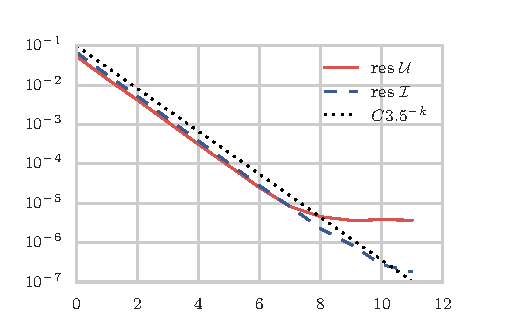
\includegraphics{figures/unloaded_error}
  \caption{\label{fig:unloaded_convergece_test}Convergence of the
    backward displacement method for the unloaded
    ($\mathrm{res}\;\mathcal{U}$) and loaded
    ($\mathrm{res}\;\mathcal{I}$) geometry.}
\end{figure}


\subsubsection{Convergence of the joint estimation of unloaded
  configuration and passive material parameters}
\label{sec:convergence_unloaded_material}

In this section we want to show that the iterative approach outlined
in Algorithm \ref{alg:unload_mat_bdm} is able to retrieve a known
material parameter under ideal circumstances. Further, we would like
to analyze the stability of the method with respect to noise in the
measurements.

A simple ellipsoidal geometry is inflated first to 0.6 kPa and then
to 1 kPa using known material parameters. Here we choose $a=3.1268$
kPa, $a_f = 1$ kPa, $b=1.0$ and $b_f=1.0$. At the first point with a
pressure of 0.6 kPa, the geometry is saved and will be used as the image-based
geometry. The second point, with the pressure at 1 kPa will represent
the end-diastolic state, and the cavity volume is computed.

We start the joint estimation with an initial guess for $a$ of 30
kPa. The relative error in the material
parameter is shown for each iteration in Figure
\ref{fig:unloaded_materror}. Here we also plot the chosen residual, which
is the relative difference in unloaded cavity volumes in two
successive iterations. We note that both of these residuals
converges at the same rate. 


\begin{figure}[htbp]
  \centering
  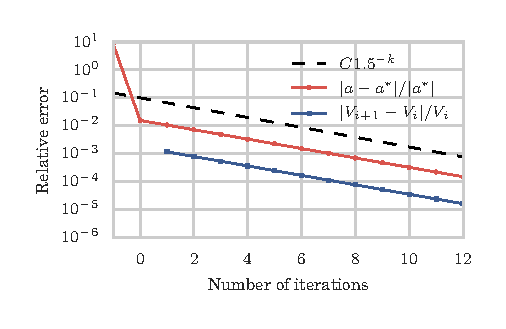
\includegraphics{figures/materror}
  \caption{\label{fig:unloaded_materror}Relative error in the material parameter for each iteration
  (red curve). The first point, at iteration -1 represent the error in
  the initial guess which is set to 30 kPa. The second point
  represents the error after estimating the material parameter by
  subtracting the offset. The remaining points represents the error
  after first unloading, and then optimizing with respect to the
  end-diastolic volume. Here we also show the chosen residual, which
  is the relative difference in unloaded cavity volumes (blue curve) and a
  supporting line showing the order of convergence. }
\end{figure}

To see the effect of noise in the data, we also test the method after
adding noise to the volume and pressure measurements. More specifically, we add
$\pm$ 0.1, 1, 5 and 10 $\%$ error to the pressure and volumes
independently. The resulting relative deviation from the exact value of the
material parameter is shown in Figure
\ref{fig:unloaded_materror_noise} for each iteration. We note that the
relative error in the resulting material parameter is of the same
order as noise level.

\begin{figure}[htbp]
  \centering
    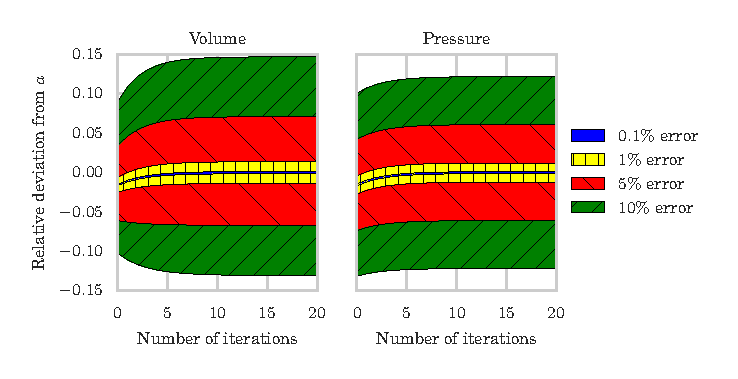
\includegraphics{figures/materror_noise}
   \caption{\label{fig:unloaded_materror_noise}  Relative deviation from the
     exact value of the material parameter when noise is added
     to the measured volumes (left)
     and pressure (right). Noise of 0.1, 1, 5 and 10 $\%$
     is added and subtracted from the target volume and pressure, and
     the material parameter is estimated using Algorithm
     \ref{alg:unload_mat_bdm}. On the $y-$axis we show the
     relative deviation from the exact value, plotted against the number
   of iterations on the $x-$axis. }
\end{figure} 
% We want to test the accuracy of the proposed method for estimating
% material parameters and the unloaded configuration. To do this we 

% \begin{figure}[htbp]
%   \begin{subfigure}[t]{\textwidth}
%     \includegraphics[width=\textwidth]{../convergence_tests/unloaded_material_parameter_estimaton/material_parameter}
%     \caption{\label{fig:unloaded_material_parameter_value}} 
%   \end{subfigure}
%   \begin{subfigure}[t]{\textwidth}
%     \includegraphics[width=\textwidth]{../convergence_tests/unloaded_material_parameter_estimaton/material_parameter_error}
%     \caption{\label{fig:unloaded_material_parameter_error}} 
%   \end{subfigure}
% \caption{\label{fig:material_control}} 
% \end{figure}

\newpage


% \bibliographystyle{spbasic}
\bibliographystyle{plain}
\bibliography{chapters/paper4/bibliography}


%  LocalWords:  subendocardial

%%% Local Variables:
%%% mode: latex
%%% TeX-master: "../../main"
%%% End:
